\section{Allenamento della rete}
Per allenare le reti \`e stato scelto l'algoritmo di Back Propagation. L'aggiornamento dei pesi viene fatto in batchlearning, ovvero alla fine di tutte le sessioni, per la rete neurale ricorrente e on-line, cio\`e alla fine di ogni sessione, per la rete neurale non ricorrente. Sono stati utilizzati diversi valori di learning rate e di momentum, due parametri che influiscono su come la rete \`e allenata; il primo \`e una costante che decide la quantit\`a di cambiamento sui vecchi pesi all'interno della rete mentre il secondo comporta un ulteriore adattamento dei pesi in base ai cambiamenti precedenti e permette di avvicinarsi pi\`u velocemente al minimo.\\
Dopo diverse prove sono stati utilizzati valori i seguenti valori:
\begin{table}[ht]
\centering
\begin{tabular}{| c | c | c |}
\multicolumn {3}{c}{}\\
\hline
&\textbf{FFN}&\textbf{RNN}\\\hline
Learning Rate&0.3&0.1\\\hline
Momentum&0.9&0.3\\\hline
\end{tabular}
\end{table}
\\

\subsection{Back Propagation}
L'algoritmo di Back Propagation \`e utilizzato con l'apprendimento supervisionato, ovvero dove insieme all'input \`e noto pure il target della funzione, e permette di modificare i pesi delle connessioni all'interno della rete in modo che venga minimizzata una certa funzione  di errore $E(w)$. L'aggiornamento dei pesi viene fatto una volta che \`e stato prodotto l'output e la quantit\`a \`e determinata dalla differenza tra lo stesso e il target (l'output reale della funzione). La funzione d'errore da minimizzare in questo esperimento \`e quella dei minimi quadrati (Mean Square Error, MSE): $E(w) =\sum\frac{1}{2}(out - tar )^2$.\\
$E(w)$ \`e una funzione nei pesi, che variano nel tempo a causa degli aggiornamenti, e per minimizzarla si utilizza l'algoritmo di discesa lungo il gradiente. Trovandosi in un punto $x_0$ viene calcolato il gradiente $\mathcal{r}f(x_0)$, cio\`e la somma delle derivate parziali in $x_0$, che d\`a indicazioni sulla direzione in cui muoversi. Giunti nel nuovo punto $x_1$, dopo essersi mossi di una certa quantit\`a $\eta$, vengono rifatti gli stessi passaggi.\\
L'algoritmo di BackPropagation pu\`o essere diviso in due parti:
\begin{itemize}
\item[-]Passo in avanti: l'input viene propagato nella rete per tutti i suoi strati fino giungere all'ultimo, dove viene prodotto l'output;
\item[-]Passo all'indietro: viene calcolato l'errore utilizzando $E(w)$ che viene propagato dall'output fino all'input e i pesi vengono aggiornati appropriatamente.
\end{itemize}
Quando si aggiornano i pesi si tiene conto anche del \emph{learning rate} $\mu$, un valore che influisce sulla velocit\`a e sulla qualit\`a dell'apprendimento: pi\`u basso \`e il valore pi\`u lento ma preciso sar\`a l'allenamento della rete, pi\`u altro \`e il valore pi\`u veloce ma impreciso sar\`a l'allenamento.


\subsection{Bold Driver}
\begin{figure}[!htb]
\centering
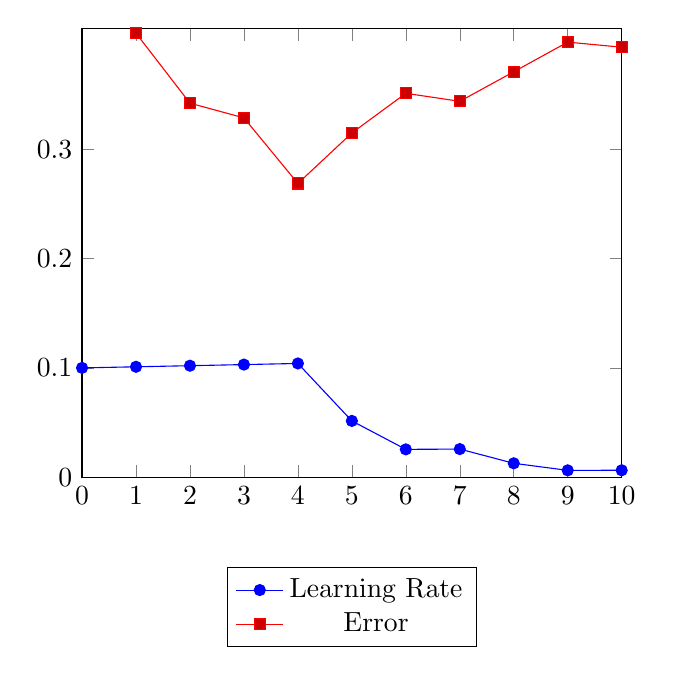
\begin{tikzpicture}
\begin{axis}[
xmin=0, xmax=10,
ymin=0, ymax=0.41,
xtick={0,1,2,3,4,5,6,7,8,9,10},
ytick={0,0.1,0.2,0.3},
legend style={at={(0.5,-0.2)},anchor=north} % Put the legend below the plot
]
\addplot[mark=*,blue]
coordinates {(0,0.1)(1,0.101)(2,0.10201)(3,0.1030301)(4,0.104060)(5,0.051509)(6,0.025497)(7,0.025752)(8,0.012747)(9,0.00630)(10,0.006373)};
\addlegendentry{Learning Rate}
\addplot
coordinates {(0,0.5)(1,0.406092)(2,0.342092)(3,0.328655)(4,0.268666)(5,0.314834)(6,0.351122)(7,0.343793)(8,0.370810)(9,0.397950)(10,0.393275)};
\addlegendentry{Error}
\end{axis}
\end{tikzpicture}
\caption{Il grafico illustra la variazione del learning rate in una sessione di allenamento;}
\label{fig:lr}
\end{figure}
Per manipolare il valore del learning rate \`e stata adottata la tecnica Bold Driver~\cite{battiti1989accelerated} che ne cambia la quantit\`a a seconda di come procede l'apprendimento da parte della rete. Si confrontano gli errori al tempo $t$ e $t-1$ e in base ai loro valori viene fatto un cambiamento:
\begin{itemize}
\item[-]se l'errore \`e diminuito si aumenta $\mu$ di una quantit\`a pari all'uno per cento del suo valore;
\item[-]se l'errore \`e aumentato si annulla l'ultimo cambiamento fatto e si diminuisce $\mu$ del suo 50\%.
\end{itemize}
L'andamento del learning rate in uno degli esperimenti eseguiti, specificamente il primo utilizzando una RNN, \`e illustrato nella figura~\ref{fig:lr}.\\

\subsection{Momentum}
Il \emph{momentum} \`e un'estensione dell'algoritmo di BackPropagation che, aggiungendo una costante $0 \le m \le 1$ all'aggiornamento dei pesi, in alcuni casi pu\`o permettere di muoversi pi\`u velocemente verso il minimo. Quando il gradiente mantiene approsimativamente la stessa direzione il \emph{momentum} aumenta la grandezza dei passi effettuati. \`E da notare che, in caso di valori molto alti, va usato un valore di $\mu$ molto piccolo, altrimenti si rischia di saltare il minimo perch\`e i passi effettuati nella discesa lungo il gradiente sono troppo grandi.


\subsection{Funzione utilizzata per l'allenamento}
Per allenare la rete \`e stata utilizzata la tecnica di k-fold cross validation~\cite{kohavi1995study}, dividendo il database iniziale in dieci parti ed utilizzandone nove per l'allenamento e una per la validazione. Il codice riportato \`e la funzione di allenamento utilizzata per allenare la rete; \`e stata modificata dal codice originale per adattarsi meglio al programma e per implementare la k-fold cross validation.\\

\begin{lstlisting}[language=Python, caption=Train Until Convergence]
trainingData = datasetTrain
validationData = datasetTest
self.ds = trainingData
bestweights = self.module.params.copy()
bestverr = self.testOnData(validationData)
trainingErrors = []
validationErrors = [bestverr]
while True:
	trainingErrors.append(self.train())
	validationErrors.append(self.testOnData(validationData))
	if validationErrors[-1] < bestverr:
 		# one update is always done
		bestverr = validationErrors[-1]
		bestweights = self.module.params.copy()

	if maxEpochs is not None and epochs >= maxEpochs:
		self.module.params[:] = bestweights
		break
	epochs += 1

	if len(validationErrors) >= continueEpochs * 2:
		old = validationErrors[-continueEpochs * 2:-continueEpochs]
		new = validationErrors[-continueEpochs:]
		if min(new) > max(old):
			self.module.params[:] = bestweights
			break
return trainingErrors, validationErrors
\end{lstlisting}
\newpage
La funzione salva lo stato dei pesi della rete quando, in fase di validazione, viene ottenuto un errore minore all'errore pi\`u piccolo ottenuto nelle precedenti validazioni. Inoltre se l'errore comincia a salire nuovamente controlla per quanto lo fa e, in caso, blocca l'allenamento settando i pesi a quelli che davano l'errore di validazione minore e ritorna la progressione degli errori in fase di allenamento e validazione.
Per concludere questa sezione \`e da notare che \`e stata valutata l'ipotesi di utilizzare l'algoritmo di Back Propagation Through Time~\cite{werbos1990backpropagation}, versione particolare di Back Propagation adattato per le RNN ma, non essendo presente nel pacchetto utilizzato per implementare le reti~\cite{schaul2010pybrain} e avendo una complessit\`a di implementazione elevata, non \`e stato possibile farlo.




















